\section{Intra-Domain Results}\label{sec:intra_results}

As described in \autoref{sec:results_benchmarking}, the benchmark on a dataset
consisting purely of sketches is meant to remove the edge detection
preprocessing steps as possible biases. The pipeline configurations used are
the global LUMA+MEAN variant (\autoref{fig:pipeline_global_luma_mean}) and the
local LUMA+PMEAN pipeline (\autoref{fig:pipeline_local_luma_pmean}). As the two
graphs in \autoref{fig:results_precision} show, both descriptors exhibit a
large variation of precision values across the different categories. The mean
average precision shows a small advantage of the global descriptor with
$MAP=0.150$ over the local variant with $MAP=0.129$.

\autoref{fig:results_average_precision} breaks the results down and displays
the average precision for each category. Here, it is apparent, that both
descriptors deal well with some categories like "calculator", "pear" or "donut",
while the average precision values for the "parrot" or "door handle" categories
stay well below $0.05$. \autoref{fig:results_sketch_examples} displays a few
examples from two successful categories and two "difficult" categories. This is
in line with the observations made by the creators of the benchmark dataset
\autocite{eitz_how_2012}, that state that the images appear to be of varying
difficulty for computational classification. 

\begin{figure}[h]
    \centering
    \subfloat[Precisions for global LUMA+MEAN]{%
        \pgfplotstableread[]{results/pr_g_luma_mean.csv}\resultsprglumamean
\begin{tikzpicture} %[trim axis left, trim axis right]
    \begin{axis}[
        small,
        no markers,
        xmin=0.1,
        xmax=1,
        ymin=0,
        xlabel=Recall,
        ylabel=Precision,
        legend entries={
            Mean,
            Category Skull,
            Category Pear,
            Category Squirrel
        },
        ymajorgrids,
        legend style={font=\tiny},
        legend pos=outer north east,
        cycle list name=exotic,
        ]
        \addplot+[draw=none, stack plots=y, no markers, forget plot] table[x=recall, y=min]{\resultsprglumamean};
        \addplot+[draw=none, stack plots=y, fill=gray!20, no markers, forget plot] table[x=recall, y expr=\thisrow{max}-\thisrow{min}]{\resultsprglumamean} \closedcycle;
        \addplot+[stack plots=false, thick] table[x=recall, y=precision]{\resultsprglumamean};
        \addlegendentryexpanded{Mean}
        \pgfplotsinvokeforeach{skull,pear,squirrel,cabinet,pumpkin,donut}{
            \addplot+ table[x=recall, y=#1]{\resultsprglumamean};
            \addlegendentryexpanded{Category "#1"}
        }

    \end{axis}
\end{tikzpicture}

        \label{fig:results_precision_global_luma_mean}
    }
    \quad
    \subfloat[Precisions for local LUMA+PMEAN]{%
        \pgfplotstableread[]{results/pr_l_luma_pmean.csv}\resultsprllumapmean
\begin{tikzpicture} %[trim axis left, trim axis right]
    \begin{axis}[
        small,
        no markers,
        xmin=0.1,
        xmax=1,
        ymin=0,
        xlabel=Recall,
        ylabel=Precision,
        legend entries={
            Mean,
            Category Skull,
            Category Pear,
            Category Squirrel
        },
        ymajorgrids,
        legend style={font=\tiny},
        legend pos=outer north east,
        cycle list name=exotic,
        ]
        \addplot+[draw=none, stack plots=y, no markers, forget plot] table[x=recall, y=min]{\resultsprllumapmean};
        \addplot+[draw=none, stack plots=y, fill=gray!20, no markers, forget plot] table[x=recall, y expr=\thisrow{max}-\thisrow{min}]{\resultsprllumapmean} \closedcycle;
        \addplot+[stack plots=false, thick] table[x=recall, y=precision]{\resultsprllumapmean};
        \addlegendentryexpanded{Mean}
        \pgfplotsinvokeforeach{skull,pear,squirrel,cabinet,pumpkin,donut}{
            \addplot+ table[x=recall, y=#1]{\resultsprllumapmean};
            \addlegendentryexpanded{Category "#1"}
        }

    \end{axis}
\end{tikzpicture}

        \label{fig:results_precision_local_luma_pmean}
    }
    \caption[Precision and Recall Results]{
        The graphs show results of applying the global LUMA+MEAN
        \subref{fig:results_precision_global_luma_mean} and local LUMA+PMEAN
        \subref{fig:results_precision_local_luma_pmean} pipelines to
        intra-domain retrieval of sketches. The areas indicate the overall
        spread of values across all categories while the line plots show
        results for selected categories.
    }
    \label{fig:results_precision}
\end{figure}

\begin{figure}[h]
    \centering
    \pgfplotstableread[]{results/ap_g_luma_mean_l2.csv}\resultsapglumameaneucl
\pgfplotstableread[]{results/ap_g_luma_mean_cos.csv}\resultsapglumameancos
\pgfplotstableread[]{results/ap_l_luma_pmean.csv}\resultsapllumapmean
\pgfplotstableread[]{results/ap_l_luma_pmean2.csv}\resultsapllumapmeantwo
\begin{tikzpicture} %[trim axis left, trim axis right]
    \begin{axis}[
        xbar=0.2pt,
        small,
        width=\textwidth,
        y=2.4ex,
        xmin=0,
        enlarge y limits={abs=1},
        xlabel={Average Precision},
        ylabel=Category,
        ylabel near ticks,
        xlabel near ticks,
        xtick={0,0.1,...,1},
        ytick=data,
        yticklabels from table={\resultsapglumameaneucl}{query},
        yticklabel style={
            font=\tiny,
        },
        xmajorgrids,
        legend entries={
            {global LUMA+MEAN+L2},
            {global LUMA+MEAN+COS},
            {local LUMA+PMEAN},
            {local LUMA+PMEAN2},
        },
        legend style={font=\tiny},
        %legend pos=outer north east,
        bar width=2pt,
        ]
        \addplot table[y expr=-\coordindex, x=average] {\resultsapglumameaneucl};
        \addplot table[y expr=-\coordindex, x=average] {\resultsapglumameancos};
        \addplot table[y expr=-\coordindex, x=average] {\resultsapllumapmean};
        \addplot table[y expr=-\coordindex, x=average] {\resultsapllumapmeantwo};
    \end{axis}
\end{tikzpicture}

    \caption[Average Precision by Category]{
        The average precision of the LUMA+MEAN and LUMA+PMEAN pipelines broken
        down by query category.
    }
    \label{fig:results_average_precision}
\end{figure}

\begin{figure}[h!]
    \centering
    \subfloat[]{%
        \begin{tabular}{ccc}
            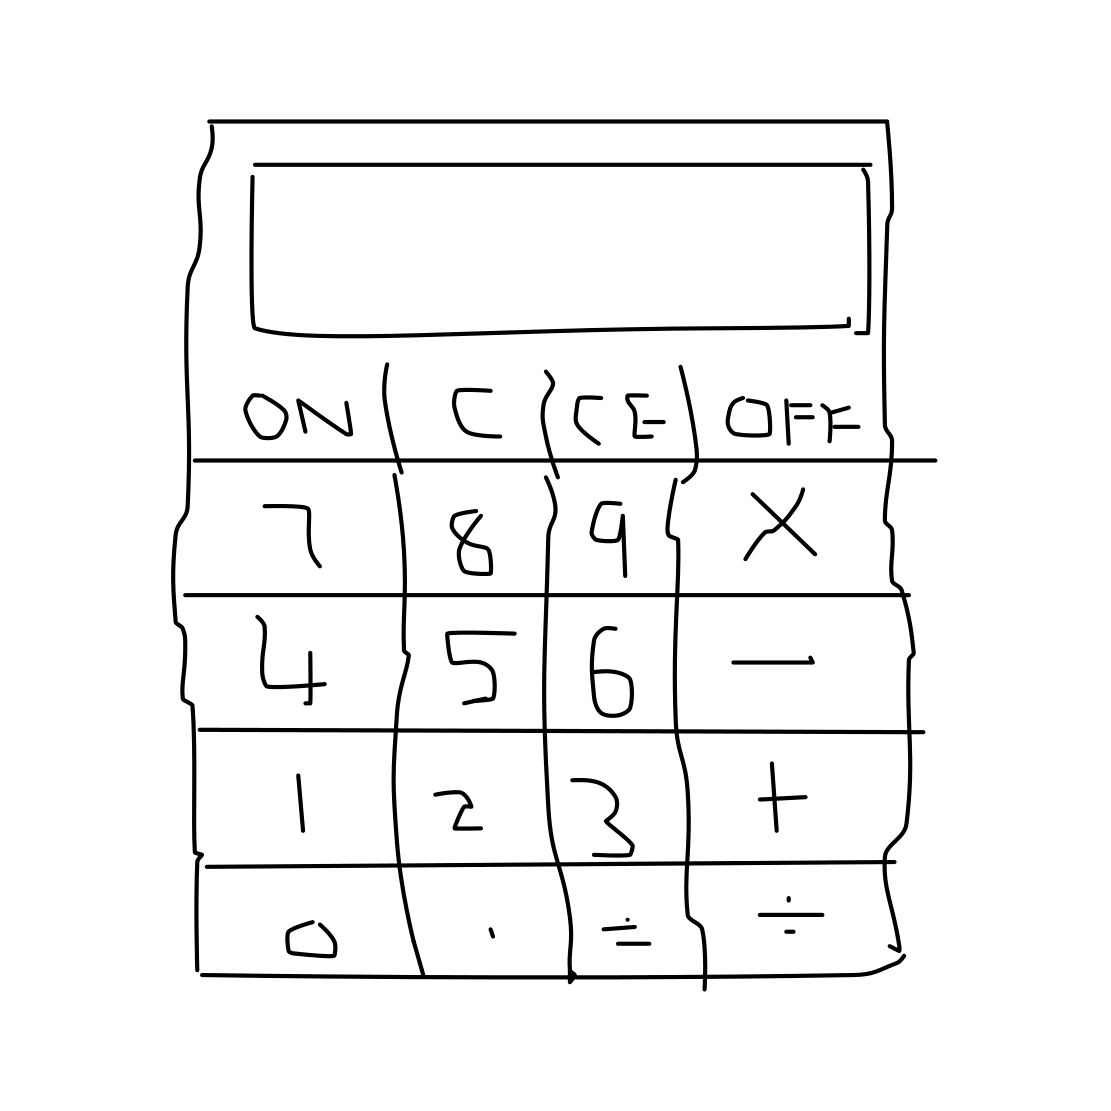
\includegraphics[width=0.15\textwidth]{illustrations/sketch_examples/calculator_1.png} &
            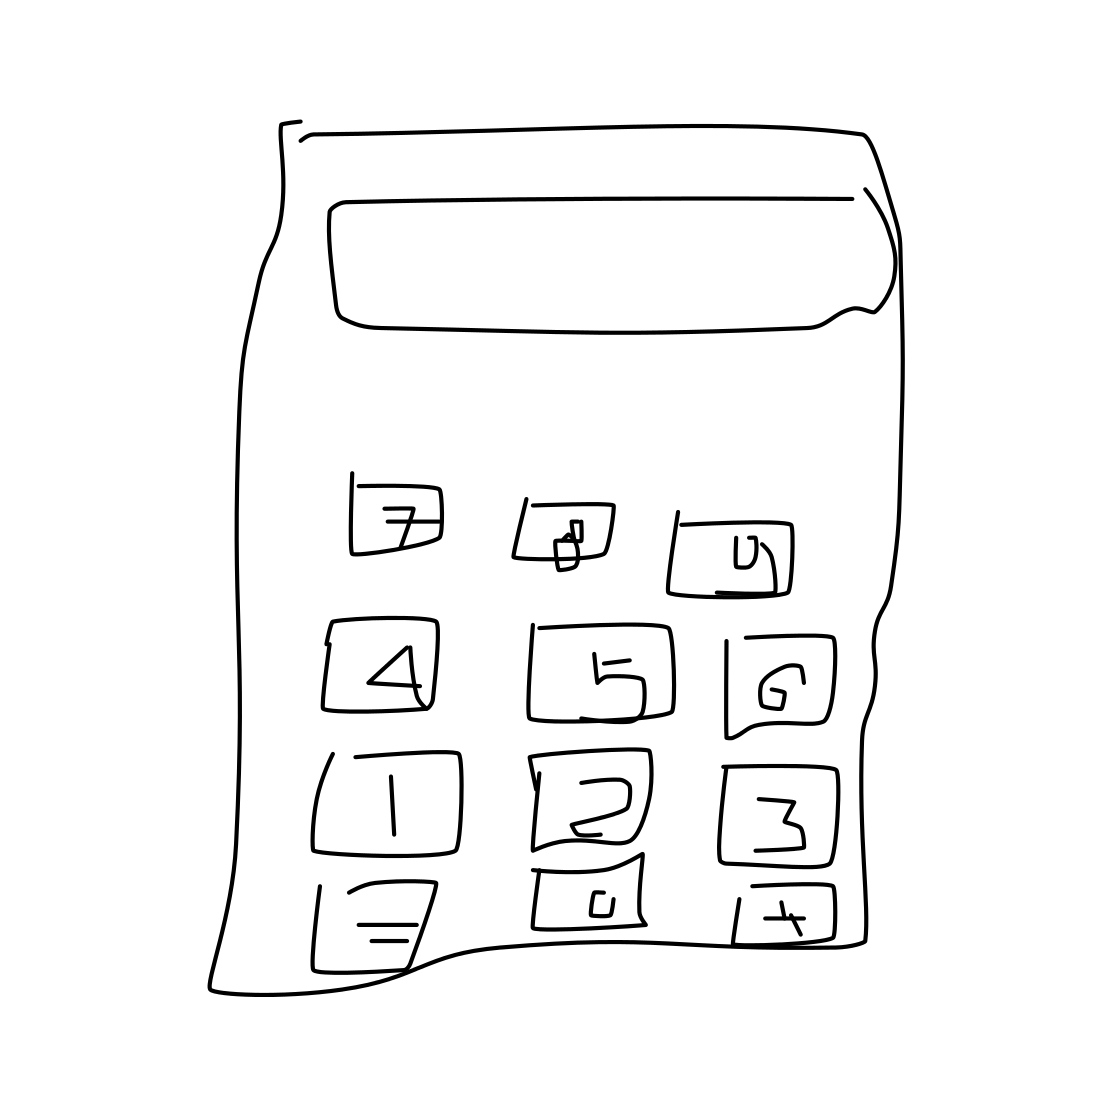
\includegraphics[width=0.15\textwidth]{illustrations/sketch_examples/calculator_2.png} &
            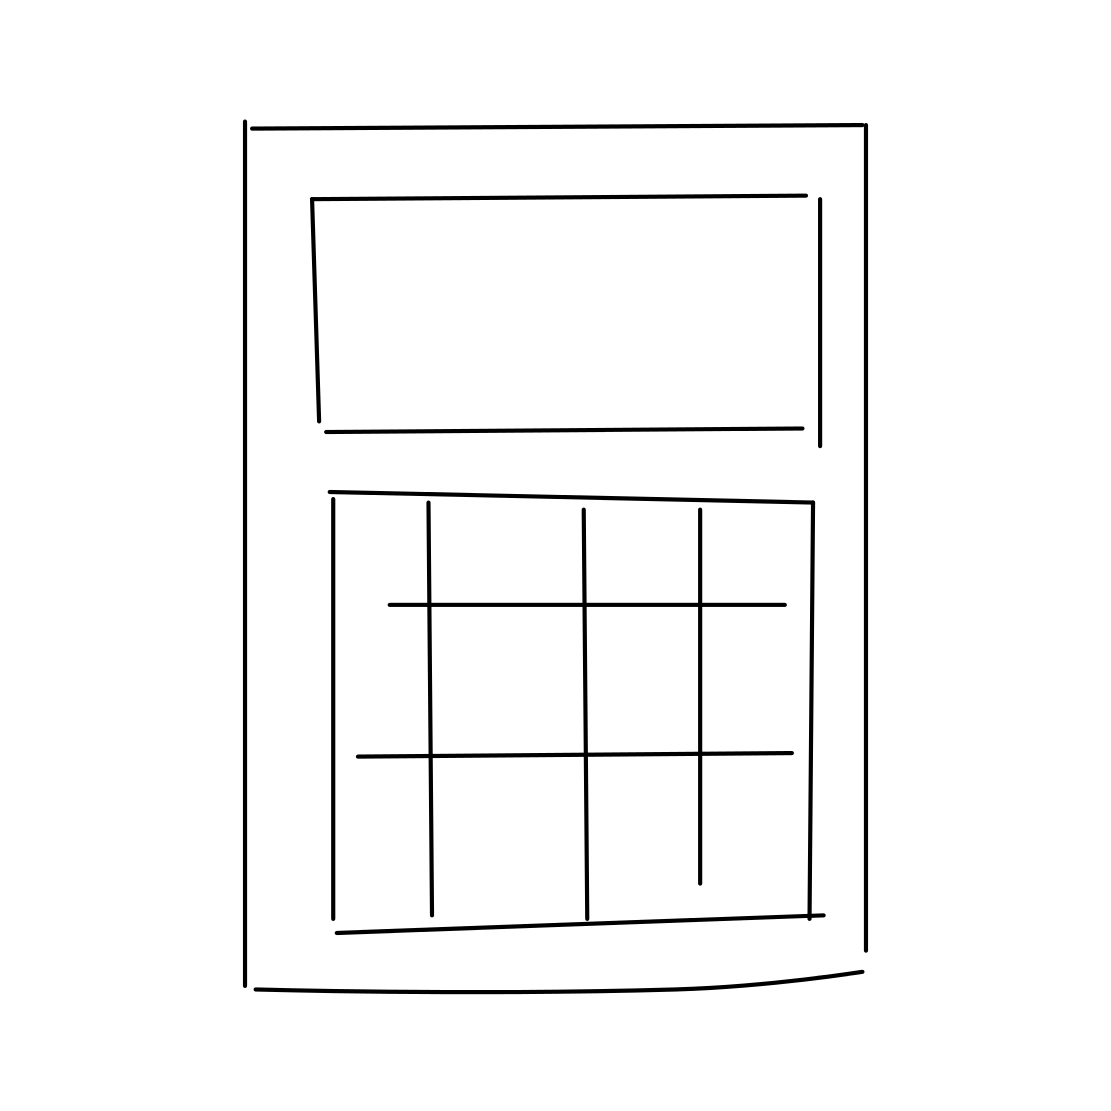
\includegraphics[width=0.15\textwidth]{illustrations/sketch_examples/calculator_3.png} \\
            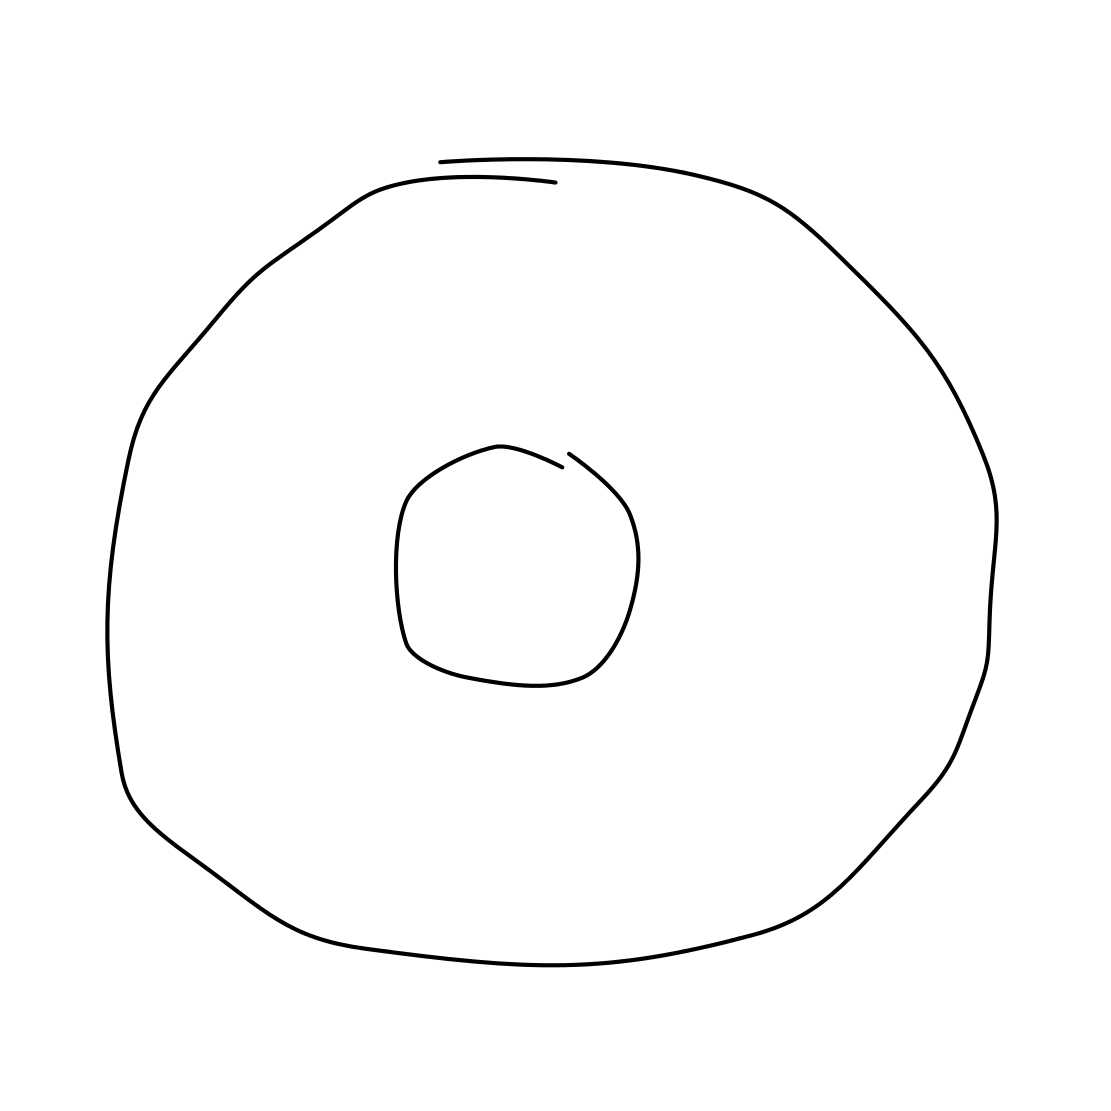
\includegraphics[width=0.15\textwidth]{illustrations/sketch_examples/donut_1.png} &
            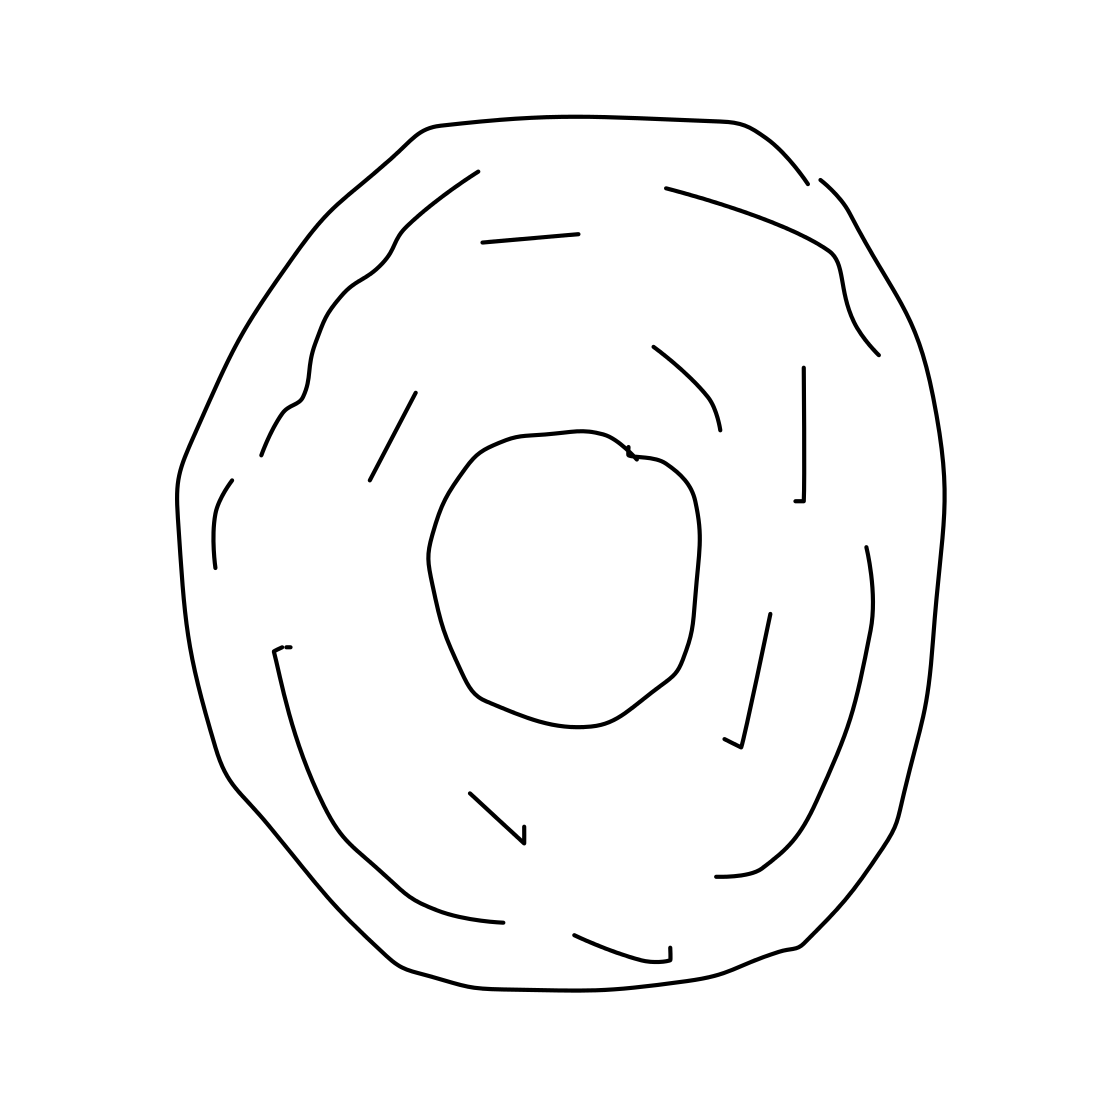
\includegraphics[width=0.15\textwidth]{illustrations/sketch_examples/donut_2.png} &
            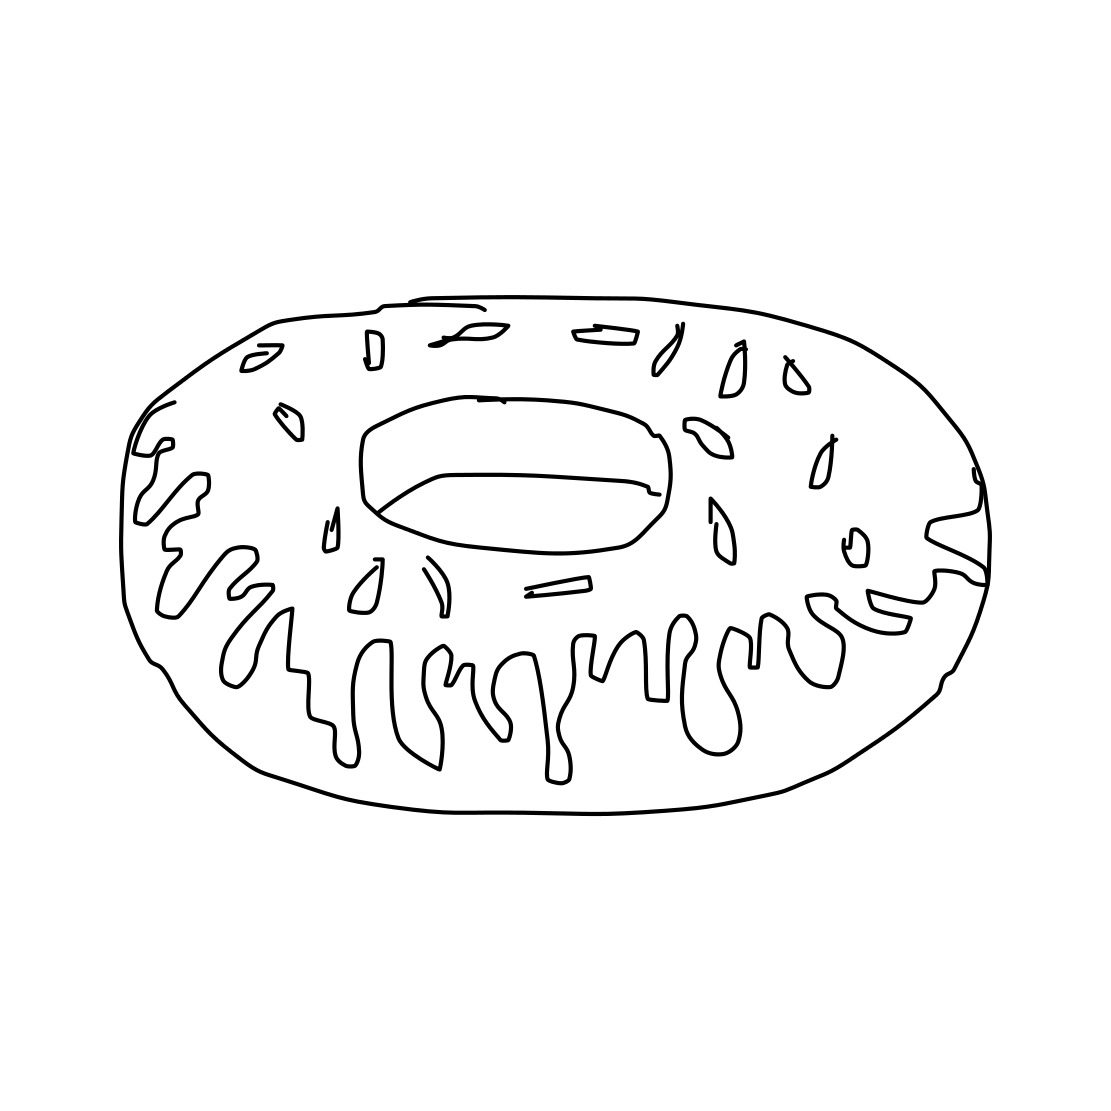
\includegraphics[width=0.15\textwidth]{illustrations/sketch_examples/donut_3.png}
        \end{tabular}
        \label{fig:results_sketch_examples_good}
    }
    \subfloat[]{%
        \begin{tabular}{ccc}
            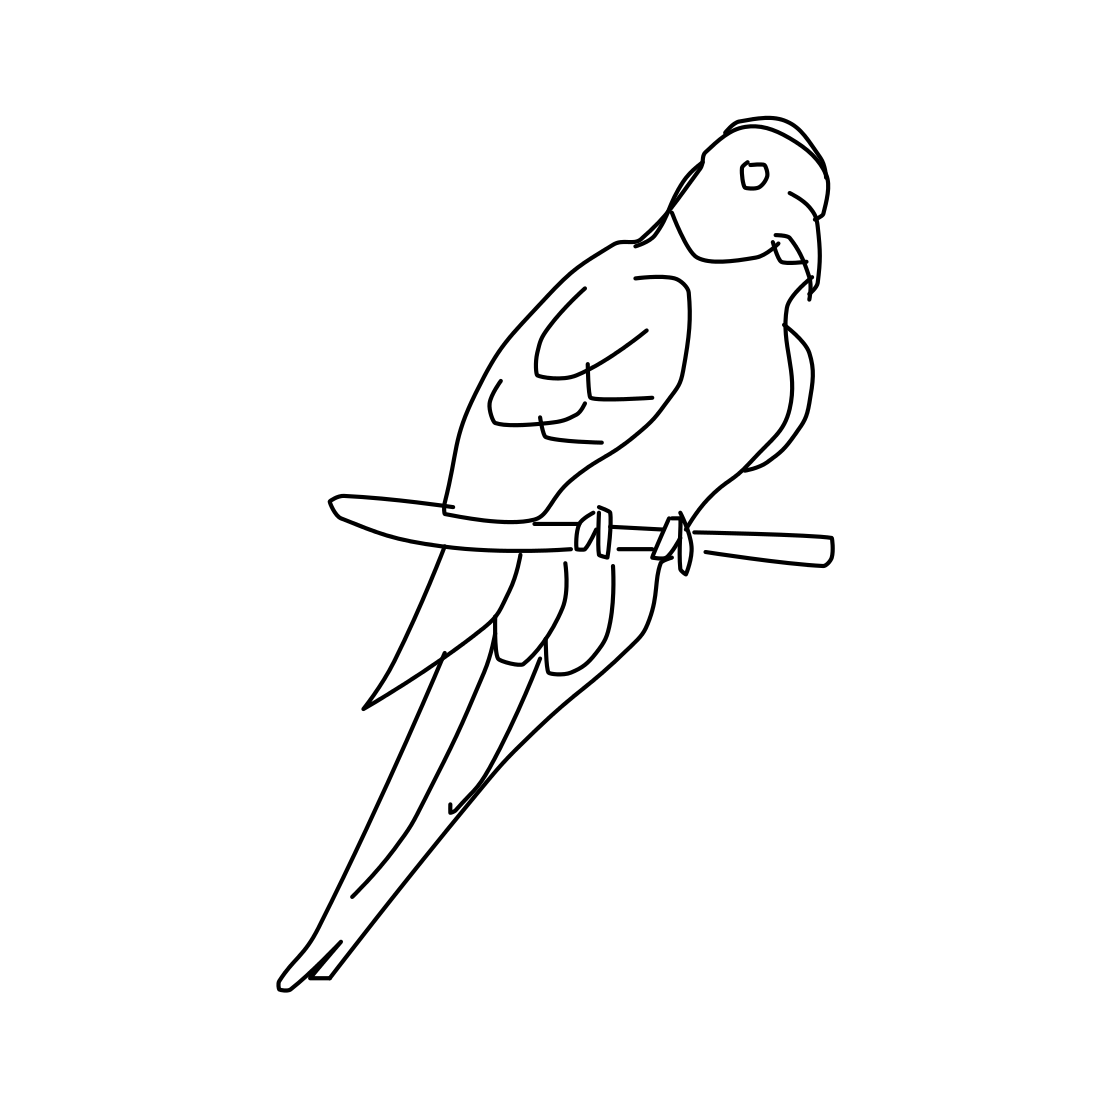
\includegraphics[width=0.15\textwidth]{illustrations/sketch_examples/parrot_1.png} &
            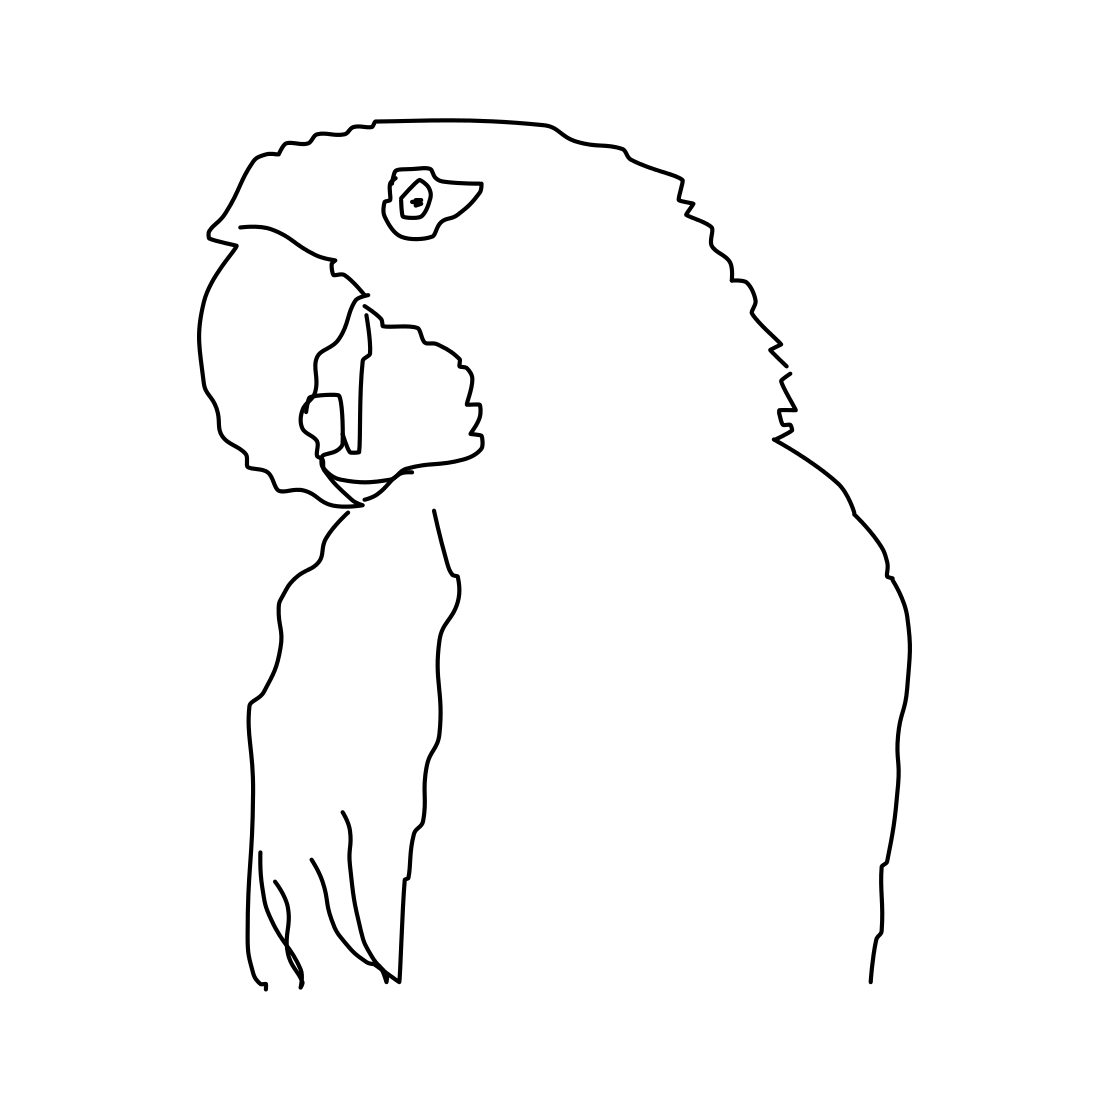
\includegraphics[width=0.15\textwidth]{illustrations/sketch_examples/parrot_2.png} &
            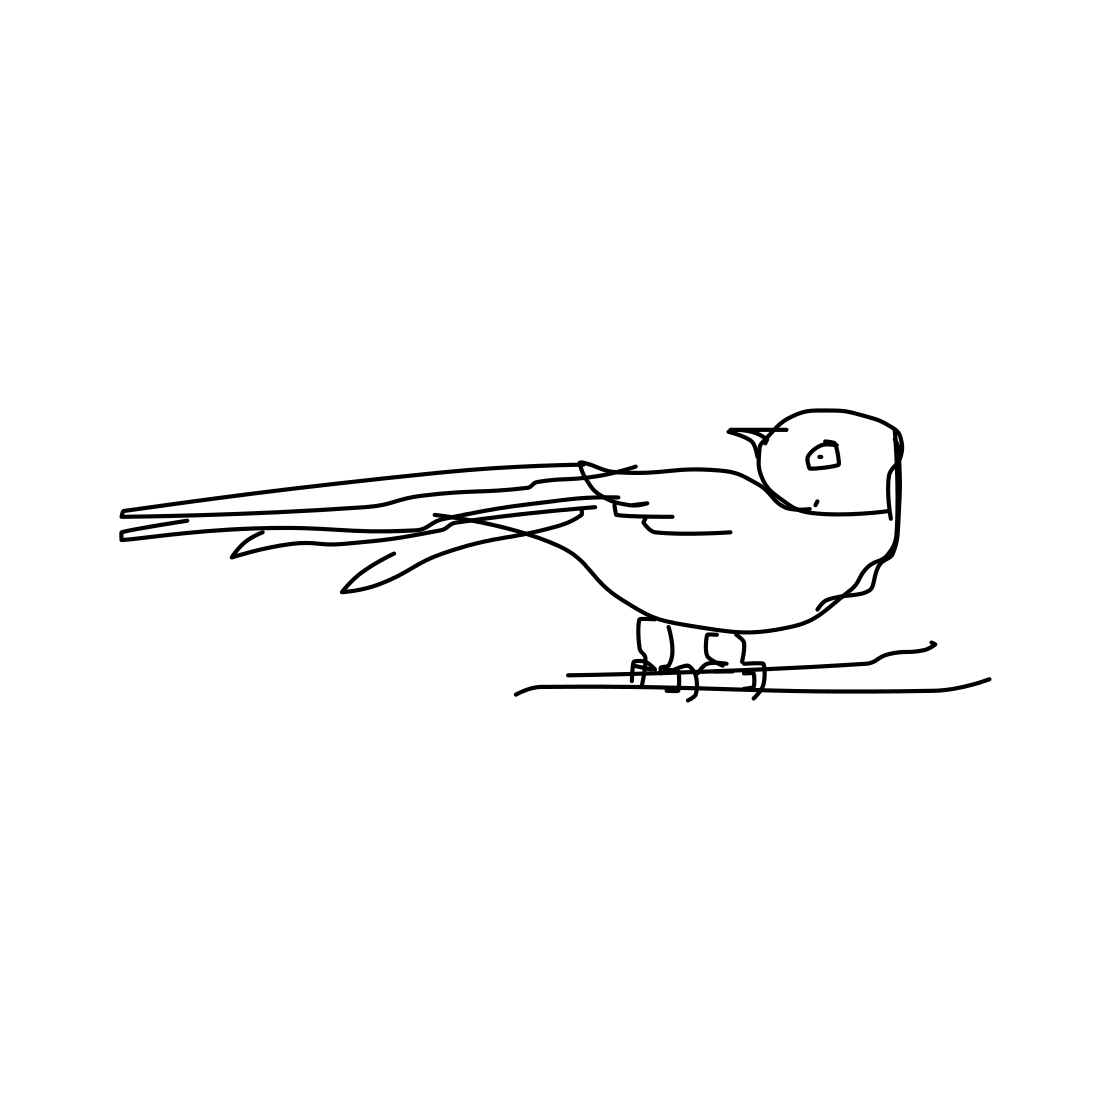
\includegraphics[width=0.15\textwidth]{illustrations/sketch_examples/parrot_3.png} \\
            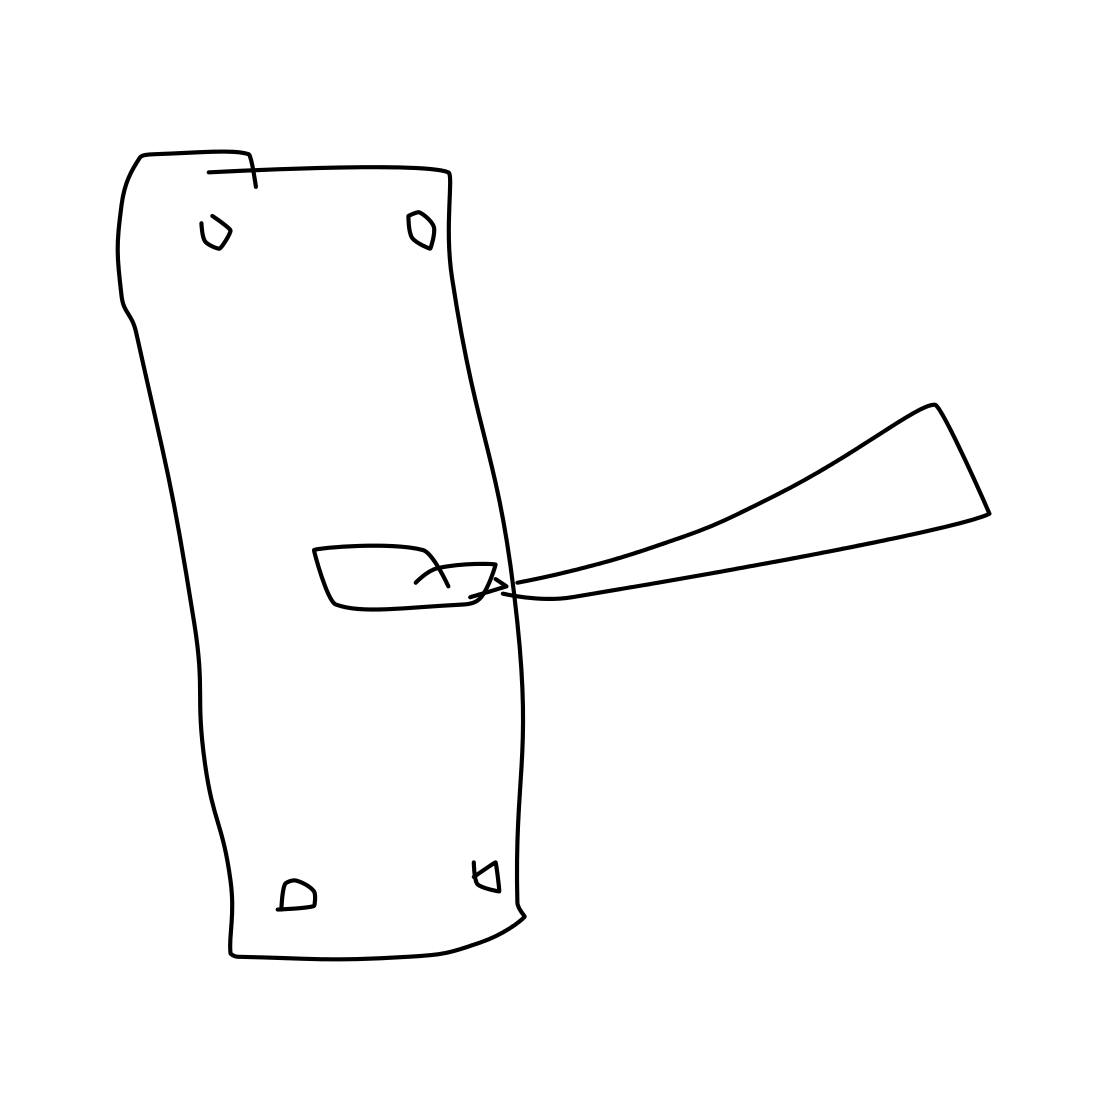
\includegraphics[width=0.15\textwidth]{illustrations/sketch_examples/doorhandle_1.png} &
            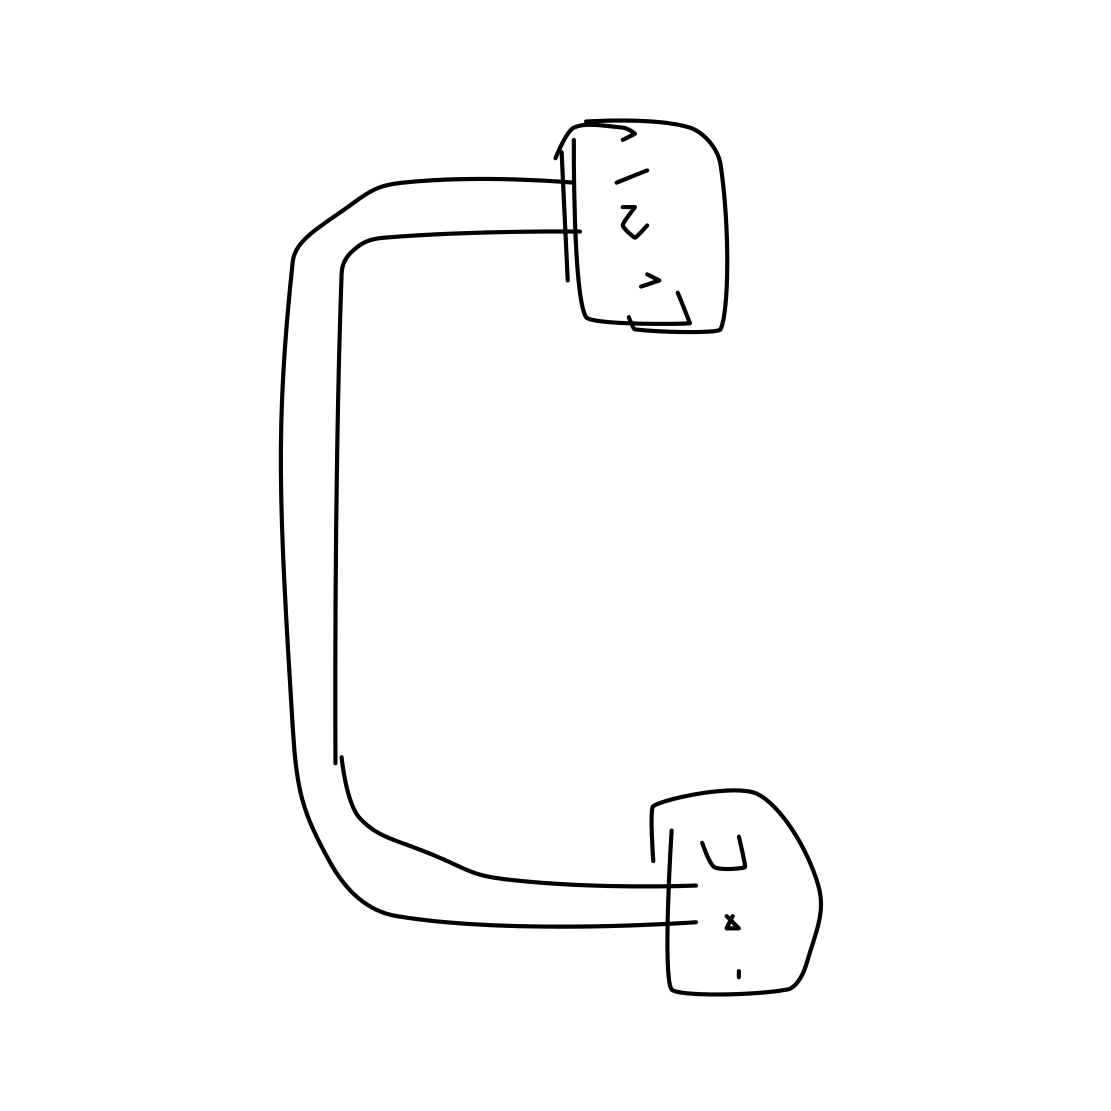
\includegraphics[width=0.15\textwidth]{illustrations/sketch_examples/doorhandle_2.png} &
            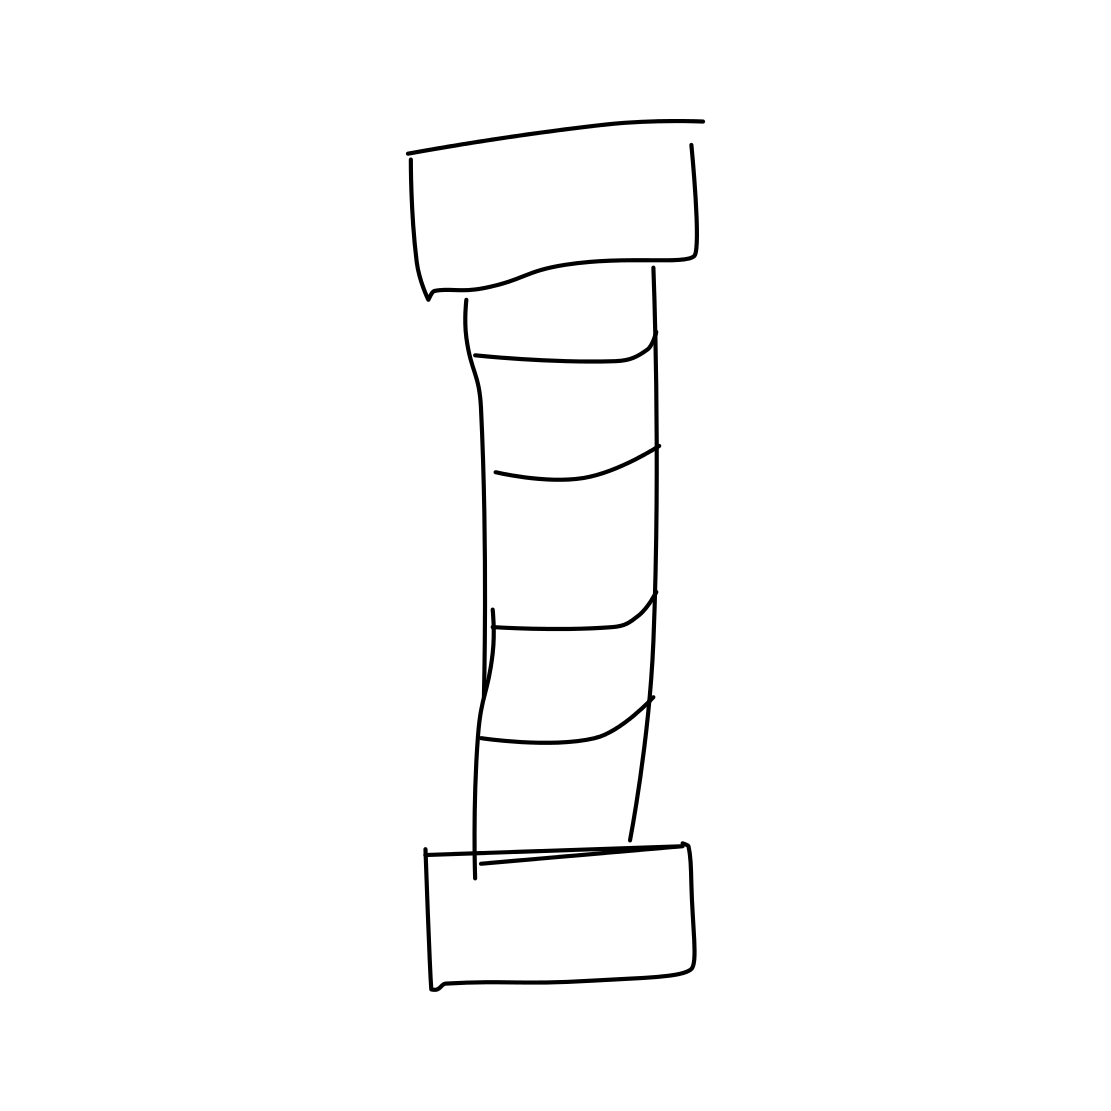
\includegraphics[width=0.15\textwidth]{illustrations/sketch_examples/doorhandle_3.png}
        \end{tabular}
        \label{fig:results_sketch_examples_bad}
    }
    \caption[Category Example Images]{
        The descriptors perform well on the categories "calculator" and "donut"
        \subref{fig:results_sketch_examples_good}, which exhibit a high degree of
        symmetry. The sketches from the categories "parrot" and "door handle"
        \subref{fig:results_sketch_examples_bad} don't have a uniform
        orientation or perspective.
    }
    \label{fig:results_sketch_examples}
\end{figure}
\FloatBarrier
